\begin{spacing}{1}
    \chapter*{Abstract}
\end{spacing}
\begin{wrapfigure}{r}{0.35\textwidth}
    \begin{center}
      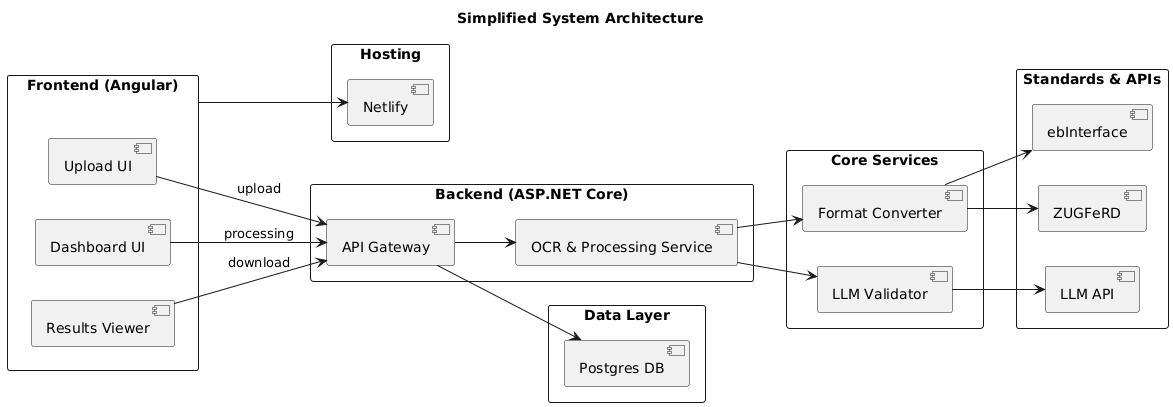
\includegraphics[width=0.33\textwidth]{pics/system-architecture.png}
    \end{center}
\end{wrapfigure}
Manual data entry of incoming invoices is a time-consuming and error-prone process.
The \textit{SmartBillConverter} was developed for PROGRAMMIERFABRIK GmbH to automate this workflow.
The system accepts invoices in a variety of input formats -- both native PDF files and scanned images -- and converts them into two standardised machine-readable XML formats: \textit{ebInterface~6.1}, the Austrian national e-invoicing standard maintained by AUSTRIAPRO, and \textit{ZUGFeRD~2.3}, a European hybrid format that embeds structured XML data inside a human-readable PDF/A-3 document.

The processing pipeline consists of three stages.
In the first stage, text is extracted from the input document: PdfPig is used for native PDF files, while Tesseract~4 (LSTM-based OCR) processes scanned images.
In the second stage, the extracted text is forwarded to the Gemini~2.5~Flash API; a carefully designed prompt instructs the model to output a strictly typed JSON object containing all invoice fields, while all monetary sums and tax calculations are computed deterministically in the C\# backend to prevent hallucination-induced errors.
In the third stage, separate mapper classes transform the internal data model into the respective target XML format and validate the output against both the XSD schema and the EN~16931 Schematron business rules.

The backend is implemented in ASP.NET Core~9.0, the frontend is a single-page application built with Angular, data is persisted in PostgreSQL via Entity Framework Core, and the entire stack is containerised with Docker~Compose.
All ten test invoices passed the official AUSTRIAPRO ebInterface validator and the German \textit{E-Rechnungs-Validator}. A short anonymised characterisation of the test set is provided in the appendix (Table \ref{tab:testrechnungen}).

\newpage
\begin{spacing}{1}
    \chapter*{Zusammenfassung}
\end{spacing}
\begin{wrapfigure}{r}{0.35\textwidth}
    \begin{center}
      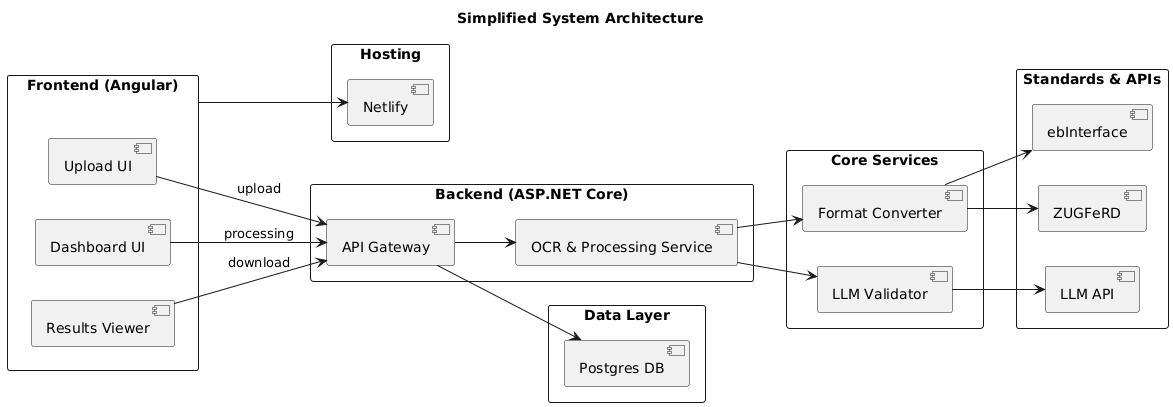
\includegraphics[width=0.33\textwidth]{pics/system-architecture.png}
    \end{center}
\end{wrapfigure}
Die manuelle Erfassung eingehender Rechnungen ist ein zeitaufwändiger und fehleranfälliger Prozess.
Der \textit{SmartBillConverter} wurde für die PROGRAMMIERFABRIK GmbH entwickelt, um diesen Arbeitsablauf zu automatisieren.
Das System nimmt Rechnungen in verschiedenen Eingabeformaten entgegen -- sowohl nativ-digitale PDFs als auch eingescannte Bilder -- und wandelt sie in zwei standardisierte, maschinenlesbare XML-Formate um: \textit{ebInterface~6.1}, den österreichischen nationalen E-Rechnungsstandard von AUSTRIAPRO, und \textit{ZUGFeRD~2.3}, ein europäisches Hybridformat, das strukturierte XML-Daten in ein menschenlesbares PDF/A-3-Dokument einbettet.

Die Verarbeitungspipeline besteht aus drei Stufen.
In der ersten Stufe wird der Text aus dem Eingabedokument extrahiert: Für native PDFs wird PdfPig verwendet, gescannte Bilder werden durch Tesseract~4 (LSTM-basierte OCR) verarbeitet.
In der zweiten Stufe wird der extrahierte Text an die Gemini~2.5~Flash API übergeben; ein sorgfältig formulierter Prompt weist das Modell an, ein streng typisiertes JSON-Objekt mit allen Rechnungsfeldern auszugeben, während alle Geldbeträge und Steuerberechnungen deterministisch im C\#-Backend berechnet werden, um Halluzinationsfehler zu verhindern.
In der dritten Stufe transformieren separate Mapper-Klassen das interne Datenmodell in das jeweilige Zielformat und validieren die Ausgabe gegen das XSD-Schema sowie die EN~16931 Schematron-Geschäftsregeln.

Das Backend ist in ASP.NET Core~9.0 implementiert, das Frontend ist eine Single-Page-Application auf Basis von Angular, die Datenpersistenz erfolgt über PostgreSQL mit Entity Framework Core, und der gesamte Stack ist mit Docker~Compose containerisiert.
Alle zehn Testrechnungen wurden von den verwendeten Validatoren akzeptiert. Eine kurze, anonymisierte Charakterisierung des Testsets ist im Anhang enthalten (Tabelle \ref{tab:testrechnungen}).
